% ---------
%  Compile with "pdflatex hw0".
% --------
%!TEX TS-program = pdflatex
%!TEX encoding = UTF-8 Unicode

\documentclass[11pt]{article}
\usepackage{jeffe,handout,graphicx}
\usepackage[utf8]{inputenc}		% Allow some non-ASCII Unicode in source
\usepackage{tikz}

% =========================================================
%   Define common stuff for solution headers
% =========================================================
\Class{CS/ECE 374}
\Semester{Spring 2023}
\Authors{1}
\AuthorOne{William Cheng}{shihuac2@illinois.edu}
%\Section{}

% =========================================================
\begin{document}

% ---------------------------------------------------------


\HomeworkHeader{3}{1}	% homework number, problem number

\begin{solution}
\begin{enumerate}[(a)]
\item The NFA is shown below.
\begin{center}
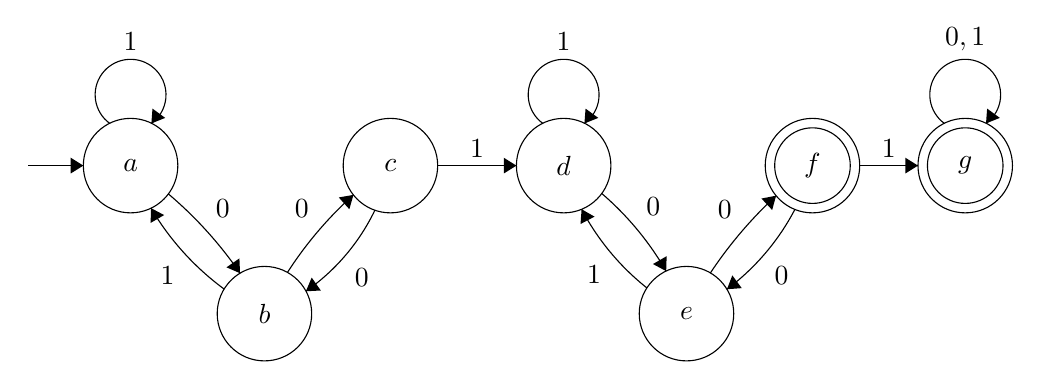
\begin{tikzpicture}[scale=0.2]
\tikzstyle{every node}+=[inner sep=0pt]
\draw [black] (9,-14.2) circle (3);
\draw (9,-14.2) node {$a$};
\draw [black] (17.5,-23.6) circle (3);
\draw (17.5,-23.6) node {$b$};
\draw [black] (25.5,-14.2) circle (3);
\draw (25.5,-14.2) node {$c$};
\draw [black] (36.5,-14.2) circle (3);
\draw (36.5,-14.2) node {$d$};
\draw [black] (44.3,-23.6) circle (3);
\draw (44.3,-23.6) node {$e$};
\draw [black] (52.3,-14.2) circle (3);
\draw (52.3,-14.2) node {$f$};
\draw [black] (52.3,-14.2) circle (2.4);
\draw [black] (62,-14.2) circle (3);
\draw (62,-14.2) node {$g$};
\draw [black] (62,-14.2) circle (2.4);
\draw [black] (2.5,-14.2) -- (6,-14.2);
\fill [black] (6,-14.2) -- (5.2,-13.7) -- (5.2,-14.7);
\draw [black] (7.677,-11.52) arc (234:-54:2.25);
\draw (9,-6.95) node [above] {$1$};
\fill [black] (10.32,-11.52) -- (11.2,-11.17) -- (10.39,-10.58);
\draw [black] (11.399,-15.998) arc (49.77753:34.46573:25.474);
\fill [black] (15.95,-21.03) -- (15.91,-20.09) -- (15.09,-20.66);
\draw (14.38,-16.9) node [right] {$0$};
\draw [black] (14.942,-22.04) arc (-126.33983:-149.41691:17.316);
\fill [black] (10.3,-16.9) -- (10.27,-17.84) -- (11.13,-17.34);
\draw (11.82,-21.16) node [left] {$1$};
\draw [black] (18.962,-20.982) arc (147.27057:131.92962:24.206);
\fill [black] (23.15,-16.06) -- (22.22,-16.22) -- (22.89,-16.97);
\draw (20.34,-16.94) node [left] {$0$};
\draw [black] (24.515,-17.027) arc (-25.67154:-55.12827:13.297);
\fill [black] (20.13,-22.18) -- (21.08,-22.13) -- (20.5,-21.31);
\draw (23.21,-21.33) node [right] {$0$};
\draw [black] (28.5,-14.2) -- (33.5,-14.2);
\fill [black] (33.5,-14.2) -- (32.7,-13.7) -- (32.7,-14.7);
\draw (31,-13.7) node [above] {$1$};
\draw [black] (35.177,-11.52) arc (234:-54:2.25);
\draw (36.5,-6.95) node [above] {$1$};
\fill [black] (37.82,-11.52) -- (38.7,-11.17) -- (37.89,-10.58);
\draw [black] (38.919,-15.969) arc (49.32206:30.04885:19.123);
\fill [black] (43.01,-20.9) -- (43.04,-19.95) -- (42.17,-20.45);
\draw (41.72,-16.83) node [right] {$0$};
\draw [black] (41.788,-21.969) arc (-128.44425:-152.18484:15.788);
\fill [black] (37.64,-16.97) -- (37.57,-17.91) -- (38.46,-17.44);
\draw (38.9,-21.12) node [left] {$1$};
\draw [black] (45.818,-21.014) arc (146.41017:132.79003:27.143);
\fill [black] (49.99,-16.11) -- (49.06,-16.29) -- (49.74,-17.02);
\draw (47.21,-17) node [left] {$0$};
\draw [black] (51.184,-16.979) arc (-27.58906:-53.21075:15.027);
\fill [black] (46.87,-22.05) -- (47.81,-21.98) -- (47.21,-21.17);
\draw (49.86,-21.2) node [right] {$0$};
\draw [black] (55.3,-14.2) -- (59,-14.2);
\fill [black] (59,-14.2) -- (58.2,-13.7) -- (58.2,-14.7);
\draw (57.15,-13.7) node [above] {$1$};
\draw [black] (60.677,-11.52) arc (234:-54:2.25);
\draw (62,-6.95) node [above] {$0,1$};
\fill [black] (63.32,-11.52) -- (64.2,-11.17) -- (63.39,-10.58);
\end{tikzpicture}
\end{center}

\begin{itemize}
\item $a$: have not seen a zero yet
\item $b$: the current length of $0$ block is odd
\item $c$: the current length of $0$ block is even
\item $d$: one block of $0$'s of even length has been seen, look for the second $0$ block
\item $e$: the current length of $0$ block is odd
\item $f$: the current length of $0$ block is even
\item $g$: exactly two blocks of $0$'s of even length has been seen
\end{itemize}

\item The NFA is shown below.
\begin{center}
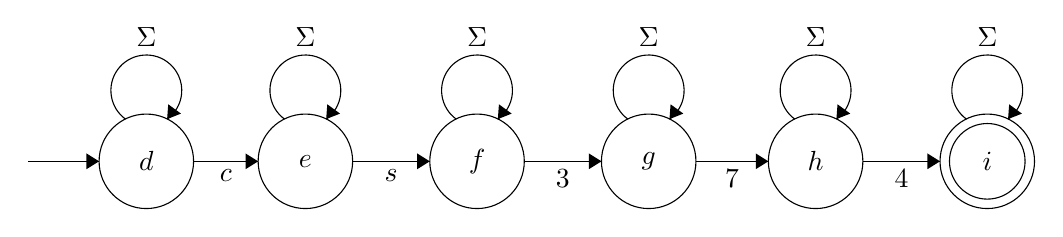
\begin{tikzpicture}[scale=0.2]
\tikzstyle{every node}+=[inner sep=0pt]
\draw [black] (11.7,-18.1) circle (3);
\draw (11.7,-18.1) node {$d$};
\draw [black] (21.8,-18.1) circle (3);
\draw (21.8,-18.1) node {$e$};
\draw [black] (32.7,-18.1) circle (3);
\draw (32.7,-18.1) node {$f$};
\draw [black] (43.6,-18.1) circle (3);
\draw (43.6,-18.1) node {$g$};
\draw [black] (54.2,-18.1) circle (3);
\draw (54.2,-18.1) node {$h$};
\draw [black] (65.1,-18.1) circle (3);
\draw (65.1,-18.1) node {$i$};
\draw [black] (65.1,-18.1) circle (2.4);
\draw [black] (4.2,-18.1) -- (8.7,-18.1);
\fill [black] (8.7,-18.1) -- (7.9,-17.6) -- (7.9,-18.6);
\draw [black] (10.377,-15.42) arc (234:-54:2.25);
\draw (11.7,-10.85) node [above] {$\Sigma$};
\fill [black] (13.02,-15.42) -- (13.9,-15.07) -- (13.09,-14.48);
\draw [black] (14.7,-18.1) -- (18.8,-18.1);
\fill [black] (18.8,-18.1) -- (18,-17.6) -- (18,-18.6);
\draw (16.75,-18.6) node [below] {$c$};
\draw [black] (24.8,-18.1) -- (29.7,-18.1);
\fill [black] (29.7,-18.1) -- (28.9,-17.6) -- (28.9,-18.6);
\draw (27.25,-18.6) node [below] {$s$};
\draw [black] (35.7,-18.1) -- (40.6,-18.1);
\fill [black] (40.6,-18.1) -- (39.8,-17.6) -- (39.8,-18.6);
\draw (38.15,-18.6) node [below] {$3$};
\draw [black] (46.6,-18.1) -- (51.2,-18.1);
\fill [black] (51.2,-18.1) -- (50.4,-17.6) -- (50.4,-18.6);
\draw (48.9,-18.6) node [below] {$7$};
\draw [black] (57.2,-18.1) -- (62.1,-18.1);
\fill [black] (62.1,-18.1) -- (61.3,-17.6) -- (61.3,-18.6);
\draw (59.65,-18.6) node [below] {$4$};
\draw [black] (20.477,-15.42) arc (234:-54:2.25);
\draw (21.8,-10.85) node [above] {$\Sigma$};
\fill [black] (23.12,-15.42) -- (24,-15.07) -- (23.19,-14.48);
\draw [black] (31.377,-15.42) arc (234:-54:2.25);
\draw (32.7,-10.85) node [above] {$\Sigma$};
\fill [black] (34.02,-15.42) -- (34.9,-15.07) -- (34.09,-14.48);
\draw [black] (42.277,-15.42) arc (234:-54:2.25);
\draw (43.6,-10.85) node [above] {$\Sigma$};
\fill [black] (44.92,-15.42) -- (45.8,-15.07) -- (44.99,-14.48);
\draw [black] (52.877,-15.42) arc (234:-54:2.25);
\draw (54.2,-10.85) node [above] {$\Sigma$};
\fill [black] (55.52,-15.42) -- (56.4,-15.07) -- (55.59,-14.48);
\draw [black] (63.777,-15.42) arc (234:-54:2.25);
\draw (65.1,-10.85) node [above] {$\Sigma$};
\fill [black] (66.42,-15.42) -- (67.3,-15.07) -- (66.49,-14.48);
\end{tikzpicture}
\end{center}
The NFA stays at the current state upon seeing any letter until it sees the next letter in $cs374$, starting from the first letter $c$. It will stay at the accepting state $i$ after seeing the whole sequence $cs374$.

\item The states $(q_1, q_2)\in Q_1\times Q_2$ are defined as follows: Each of $q_1$ or $q_2$ is in the set $\{ \epsilon,c,s,3,7,4 \}$. The state $(q_1, q_2)$ represents that $q_1$ has been seen in the sequence $cs374$ and $q_2$ has been seen in the sequence $cs473$.
\begin{itemize}
\item $\delta=$
\begin{math}
  \left\{
    \begin{array}{ll}
		((\epsilon, \epsilon), \Sigma)\to (\epsilon, \epsilon)\\
		((\epsilon, \epsilon), c)\to (c, c)\\
		((c, c), \Sigma)\to (c, c)\\
		((c, c), s)\to (s, s)\\
		((s, s), \Sigma)\to (s, s)\\
		((s, s), 3)\to (3, s)\\
		((s, s), 4)\to (s, 4)\\
		((3, s), \Sigma)\to (3, s)\\
		((3, s), 4)\to (3, 4)\\
		((3, s), 7)\to (7, s)\\
		((s, 4), \Sigma)\to (s, 4)\\
		((s, 4), 3)\to (3, 4)\\
		((s, 4), 7)\to (s, 7)\\
		((3, 4), \Sigma)\to (3, 4)\\
		((3, 4), 7)\to (7, 7)\\
		((7, s), \Sigma)\to (7, s)\\
		((7, s), 4)\to (4, 4)\\
		((s, 7), \Sigma)\to (s, 7)\\
		((s, 7), 3)\to (3, 3)\\
		((7, 7), \Sigma)\to (7, 7)\\
		((7, 7), 3)\to (7, 3)\\
		((7, 7), 4)\to (4, 7)\\
		((4, 4), \Sigma)\to (4, 4)\\
		((4, 4), 7)\to (4, 7)\\
		((3, 3), \Sigma)\to (3, 3)\\
		((3, 3), 7)\to (7, 3)\\
		((7, 3), \Sigma)\to (7, 3)\\
		((7, 3), 4)\to (4, 3)\\
		((4, 7), \Sigma)\to (4, 7)\\
		((4, 7), 3)\to (4, 3)\\
		((4, 3), \Sigma)\to (4, 3)\\
    \end{array}
  \right.
\end{math}\\
\item $s=(\epsilon, \epsilon)$
\item $A=\{ (4, 3) \}$
\end{itemize}
\emph{Explanation. }For a state $(q_1, q_2)$, if the input letter matches the next letter in $cs374$, $q_1$ gets updated; if the input letter matches the next letter in $cs473$, $q_2$ gets updated. Since state $(4,3)$ means that the $4$ in $cs374$ has been seen and the $3$ in $cs473$ has been seen, it is the only accepting state. Following is a visualization of the NFA.
\begin{center}
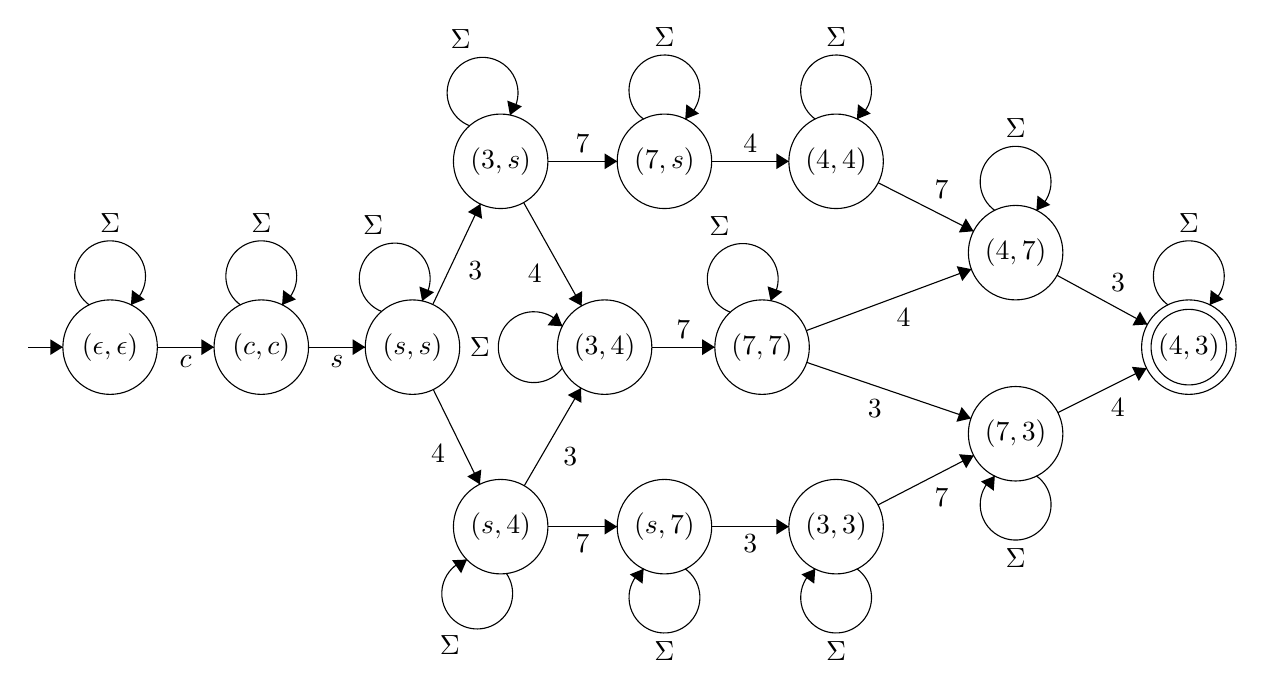
\begin{tikzpicture}[scale=0.2]
\tikzstyle{every node}+=[inner sep=0pt]
\draw [black] (6.1,-24.9) circle (3);
\draw (6.1,-24.9) node {$(\epsilon,\epsilon)$};
\draw [black] (15.7,-24.9) circle (3);
\draw (15.7,-24.9) node {$(c,c)$};
\draw [black] (25.3,-24.9) circle (3);
\draw (25.3,-24.9) node {$(s,s)$};
\draw [black] (30.9,-13.1) circle (3);
\draw (30.9,-13.1) node {$(3,s)$};
\draw [black] (30.9,-36.3) circle (3);
\draw (30.9,-36.3) node {$(s,4)$};
\draw [black] (37.5,-24.9) circle (3);
\draw (37.5,-24.9) node {$(3,4)$};
\draw [black] (41.3,-13.1) circle (3);
\draw (41.3,-13.1) node {$(7,s)$};
\draw [black] (41.3,-36.3) circle (3);
\draw (41.3,-36.3) node {$(s,7)$};
\draw [black] (47.5,-24.9) circle (3);
\draw (47.5,-24.9) node {$(7,7)$};
\draw [black] (52.2,-13.1) circle (3);
\draw (52.2,-13.1) node {$(4,4)$};
\draw [black] (52.2,-36.3) circle (3);
\draw (52.2,-36.3) node {$(3,3)$};
\draw [black] (63.6,-30.4) circle (3);
\draw (63.6,-30.4) node {$(7,3)$};
\draw [black] (63.6,-18.9) circle (3);
\draw (63.6,-18.9) node {$(4,7)$};
\draw [black] (74.6,-24.9) circle (3);
\draw (74.6,-24.9) node {$(4,3)$};
\draw [black] (74.6,-24.9) circle (2.4);
\draw [black] (4.777,-22.22) arc (234:-54:2.25);
\draw (6.1,-17.65) node [above] {$\Sigma$};
\fill [black] (7.42,-22.22) -- (8.3,-21.87) -- (7.49,-21.28);
\draw [black] (28.937,-10.846) arc (248.78443:-39.21557:2.25);
\draw (28.36,-6) node [above] {$\Sigma$};
\fill [black] (31.49,-10.17) -- (32.25,-9.61) -- (31.32,-9.24);
\draw [black] (14.377,-22.22) arc (234:-54:2.25);
\draw (15.7,-17.65) node [above] {$\Sigma$};
\fill [black] (17.02,-22.22) -- (17.9,-21.87) -- (17.09,-21.28);
\draw [black] (31.26,-39.266) arc (34.65672:-253.34328:2.25);
\draw (27.68,-43.2) node [below] {$\Sigma$};
\fill [black] (28.76,-38.39) -- (27.82,-38.43) -- (28.39,-39.26);
\draw [black] (45.496,-22.683) arc (249.85331:-38.14669:2.25);
\draw (44.79,-17.85) node [above] {$\Sigma$};
\fill [black] (48.04,-21.96) -- (48.79,-21.38) -- (47.85,-21.04);
\draw [black] (34.82,-26.223) arc (324:36:2.25);
\draw (30.25,-24.9) node [left] {$\Sigma$};
\fill [black] (34.82,-23.58) -- (34.47,-22.7) -- (33.88,-23.51);
\draw [black] (23.348,-22.638) arc (248.52133:-39.47867:2.25);
\draw (22.8,-17.79) node [above] {$\Sigma$};
\fill [black] (25.91,-21.97) -- (26.67,-21.41) -- (25.74,-21.05);
\draw [black] (42.623,-38.98) arc (54:-234:2.25);
\draw (41.3,-43.55) node [below] {$\Sigma$};
\fill [black] (39.98,-38.98) -- (39.1,-39.33) -- (39.91,-39.92);
\draw [black] (39.977,-10.42) arc (234:-54:2.25);
\draw (41.3,-5.85) node [above] {$\Sigma$};
\fill [black] (42.62,-10.42) -- (43.5,-10.07) -- (42.69,-9.48);
\draw [black] (73.277,-22.22) arc (234:-54:2.25);
\draw (74.6,-17.65) node [above] {$\Sigma$};
\fill [black] (75.92,-22.22) -- (76.8,-21.87) -- (75.99,-21.28);
\draw [black] (50.877,-10.42) arc (234:-54:2.25);
\draw (52.2,-5.85) node [above] {$\Sigma$};
\fill [black] (53.52,-10.42) -- (54.4,-10.07) -- (53.59,-9.48);
\draw [black] (53.523,-38.98) arc (54:-234:2.25);
\draw (52.2,-43.55) node [below] {$\Sigma$};
\fill [black] (50.88,-38.98) -- (50,-39.33) -- (50.81,-39.92);
\draw [black] (64.923,-33.08) arc (54:-234:2.25);
\draw (63.6,-37.65) node [below] {$\Sigma$};
\fill [black] (62.28,-33.08) -- (61.4,-33.43) -- (62.21,-34.02);
\draw [black] (62.277,-16.22) arc (234:-54:2.25);
\draw (63.6,-11.65) node [above] {$\Sigma$};
\fill [black] (64.92,-16.22) -- (65.8,-15.87) -- (64.99,-15.28);
\draw [black] (9.1,-24.9) -- (12.7,-24.9);
\fill [black] (12.7,-24.9) -- (11.9,-24.4) -- (11.9,-25.4);
\draw (10.9,-25.4) node [below] {$c$};
\draw [black] (18.7,-24.9) -- (22.3,-24.9);
\fill [black] (22.3,-24.9) -- (21.5,-24.4) -- (21.5,-25.4);
\draw (20.5,-25.4) node [below] {$s$};
\draw [black] (26.59,-22.19) -- (29.61,-15.81);
\fill [black] (29.61,-15.81) -- (28.82,-16.32) -- (29.72,-16.75);
\draw (28.81,-20.06) node [right] {$3$};
\draw [black] (26.62,-27.59) -- (29.58,-33.61);
\fill [black] (29.58,-33.61) -- (29.67,-32.67) -- (28.78,-33.11);
\draw (27.4,-31.69) node [left] {$4$};
\draw [black] (0.9,-24.9) -- (3.1,-24.9);
\fill [black] (3.1,-24.9) -- (2.3,-24.4) -- (2.3,-25.4);
\draw [black] (32.4,-33.7) -- (36,-27.5);
\fill [black] (36,-27.5) -- (35.16,-27.94) -- (36.03,-28.44);
\draw (34.85,-31.84) node [right] {$3$};
\draw [black] (32.36,-15.72) -- (36.04,-22.28);
\fill [black] (36.04,-22.28) -- (36.08,-21.34) -- (35.21,-21.83);
\draw (33.54,-20.21) node [left] {$4$};
\draw [black] (33.9,-13.1) -- (38.3,-13.1);
\fill [black] (38.3,-13.1) -- (37.5,-12.6) -- (37.5,-13.6);
\draw (36.1,-12.6) node [above] {$7$};
\draw [black] (33.9,-36.3) -- (38.3,-36.3);
\fill [black] (38.3,-36.3) -- (37.5,-35.8) -- (37.5,-36.8);
\draw (36.1,-36.8) node [below] {$7$};
\draw [black] (40.5,-24.9) -- (44.5,-24.9);
\fill [black] (44.5,-24.9) -- (43.7,-24.4) -- (43.7,-25.4);
\draw (42.5,-24.4) node [above] {$7$};
\draw [black] (44.3,-13.1) -- (49.2,-13.1);
\fill [black] (49.2,-13.1) -- (48.4,-12.6) -- (48.4,-13.6);
\draw (46.75,-12.6) node [above] {$4$};
\draw [black] (44.3,-36.3) -- (49.2,-36.3);
\fill [black] (49.2,-36.3) -- (48.4,-35.8) -- (48.4,-36.8);
\draw (46.75,-36.8) node [below] {$3$};
\draw [black] (50.34,-25.87) -- (60.76,-29.43);
\fill [black] (60.76,-29.43) -- (60.17,-28.7) -- (59.84,-29.64);
\draw (54.65,-28.18) node [below] {$3$};
\draw [black] (50.31,-23.85) -- (60.79,-19.95);
\fill [black] (60.79,-19.95) -- (59.86,-19.76) -- (60.21,-20.7);
\draw (56.48,-22.42) node [below] {$4$};
\draw [black] (54.87,-14.46) -- (60.93,-17.54);
\fill [black] (60.93,-17.54) -- (60.44,-16.73) -- (59.99,-17.62);
\draw (58.89,-15.5) node [above] {$7$};
\draw [black] (54.86,-34.92) -- (60.94,-31.78);
\fill [black] (60.94,-31.78) -- (60,-31.7) -- (60.46,-32.59);
\draw (58.89,-33.85) node [below] {$7$};
\draw [black] (66.28,-29.06) -- (71.92,-26.24);
\fill [black] (71.92,-26.24) -- (70.98,-26.15) -- (71.42,-27.05);
\draw (70.09,-28.15) node [below] {$4$};
\draw [black] (66.23,-20.34) -- (71.97,-23.46);
\fill [black] (71.97,-23.46) -- (71.5,-22.64) -- (71.02,-23.52);
\draw (70.1,-21.4) node [above] {$3$};
\end{tikzpicture}
\end{center}
\end{enumerate}
\end{solution}

% ---------------------------------------------------------
\HomeworkHeader{3}{2}

\begin{solution}
\begin{enumerate}[(a)]
\item
Let $N=(Q,\Sigma,\delta,s,A)$ be an NFA defined as follows.
\begin{itemize}
\item $Q=Q_1\times Q_2 \times \{ \text{before}, \text{in}, \text{after} \}$
\item $s=(s_1, s_2, \text{before})$
\item $A=\{ (q_1, q_2, \text{after}) \text{ } |\text{ } q_1\in A_1, q_2\in A_2 \}$
\item
$\delta((q_1, q_2, \text{before}), a)=$
\begin{math}
  \left\{
    \begin{array}{ll}
		\{ (\delta_1(q_1, a), q_2, \text{before}), (q_1, \delta_2(q_2, a), \text{in}) \} &\text{if } \delta_2(q_2,a) \neq \emptyset\\
		\{ (\delta_1(q_1, a), q_2, \text{before}) \} &\text{otherwise}
    \end{array}
  \right.
\end{math}\\\\
$\delta((q_1, q_2, \text{in}), a)=$
\begin{math}
  \left\{
    \begin{array}{ll}
		\{ (q_1, \delta_2(q_2, a), \text{in}), (\delta_1(q_1, a), q_2, \text{after}) \} &\text{if } \delta_1(q_1,a) \neq \emptyset\\
		\{ (q_1, \delta_2(q_2, a), \text{in}) \} &\text{otherwise}
    \end{array}
  \right.
\end{math}\\\\
$\delta((q_1, q_2, \text{after}), a)=\{ (\delta_1(q_1, a), q_2, \text{after}) \}$
\end{itemize}
\emph{Explanation. }$N$ non-deterministically chooses a substring $w$ in the input string. It simulates $w$ on $M_2$, and the rest of the input string on $M_1$.
\begin{itemize}
\item The state $(q_1, q_2, \text{before})$ means $N$ is simulating $M_1$, the simulation of $M_1$ is in state $q_1$, and $N$ has not extracted the substring $w$ yet.
\item The state $(q_1, q_2, \text{in})$ means $N$ is simulating $M_2$, the simulation of $M_2$ is in state $q_2$, and $N$ has already extracted the substring $w$ but not finished simulating it on $M_2$.
\item The state $(q_1, q_2, \text{after})$ means $N$ is simulating $M_1$, the simulation of $M_1$ is in state $q_1$, and $N$ has already extracted the substring $w$ and finished simulating it on $M_2$.
\end{itemize}
The NFA will reach an accepting state only if there exists a substring $w$ in the input string that is accepted by $M_2$, and the rest of the input string is accepted by $M_1$. Therefore, $N$ accepts insert$(L_1, L_2)$ by definition.

\item
\begin{enumerate}[i.]
\item
\begin{itemize}
\item $r_1=\emptyset$: $r'=\emptyset$. No strings are in $L(r_1)$ to be inserted.
\item $r_1=\epsilon$: $r'=r_2$, since $L(r')=\{\epsilon w \epsilon | w\in L(r_2)\}=L(r_2)$.
\item $r_1=a$, $a\in \Sigma$: $r'=ar_2 + r_2a$.
\end{itemize}
\item The regular expression for insert$(L(r_1), L(r_2))$ is $s'+t'$.\\
\emph{Explanation. }$L(r_1)=L(s)\cup L(t)$. Any string $xy\in L(r_1)$ is either in $L(s)$ or $L(t)$. Then for some $w\in L(r_2)$, $xwy$ either describes insert$(L(s), L(r_2))$ or insert$(L(t), L(r_2))$, therefore $s'+t'$.
\item The regular expression for insert$(L(r_1), L(r_2))$ is $s't+st'+sr_2t$.\\
\emph{Explanation. }The position for insertion is either in $s$, or in $t$, or exactly between $s$ and $t$.
\item The regular expression for insert$(L(r_1), L(r_2))$ is $s^*s's^* + s^*r_2s^*$.\\
\emph{Explanation. }The position for insertion is either in one of the $s$'s, or between two blocks (can be empty) of $s$'s.
\item Let $ins(r_1, r_2)$ be the regular expression representing the language insert$(L(r_1), L(r_2))$.
\begin{align*}
&ins(0^*+(01)^* + 011^*0, 101)\\
&= ins(0^*, 101) + ins((01)^*, 101) + ins(011^*0, 101)\\
%&= 0^*1010^* + (01)^*101(01)^* + (01)^*01011(01)^* + 101011^*0 + 0ins(11^*0, 101) + 010111^*0\\
&= 0^*1010^* + (01)^*101(01)^* + (01)^*01011(01)^* + 101011^*0 + 011^*1011^*0 + 011^*0101 + 010111^*0
\end{align*}
\end{enumerate}
\end{enumerate}
\end{solution}




\end{document}
